\subsection{Gefahrenanalyse/Studien zur menschlichen Wahrnehmung}
% Analyse von durchgeführten Studien: Inwieweit ist der Mensch anfällig für Deepfakes?
% Welche Konsequenz ergibt sich daraus? (Anforderungen an Informationen, Detektion von DF, etc.)
Folgend werden Ergebnisse mehrerer Studien betrachtet, um den Einfluss und die damit verbundenen Gefahren von Deepfakes auf den Menschen zu betrachten.
Die menschliche Wahrnehmung von Deepfakes sowie Folgen der Manipulation spielen sind dabei Hauptfaktoren.
\par
Um zu untersuchen, ob und mit welchem Umfang Deepfakes im politschen Rahmen Wähler beeinflussbar sind, manipulierten Wissenschaftler der Amsterdamer Universität Videomaterial eines holländischen Politikers (Vgl. \cite{Dobber2020}).
In diesem dreizehn sekündigen Video beinhalten die letzten fünf Sekunden manipuliertes Material in dem der folgene Satz fällt ``But, as Christ would say: don’t crucify me for it''.
Sie wählten diesen Satz, da dieser Politker einer konservativen christlichen Partei angehörte und somit die potentielle Wahlzielgruppe anspricht.
Dabei nutzte diese Studie politisches Microtargeting, ein von Parteien zur Beeinflussung von Wählern häufig gewähltes Mittel (\cite{Papakyriakopoulos2017}), indem es auf die religiöse Einstellung abzielte.
\par
An dieser Studie nahmen 277 Menschen teil, von denen 144 Teilnehmer das manipulierte Video und 133 das Originalvideo sahen.
Schlüsselfaktoren zur Einteilung und Unterscheidung waren unter anderem die Religiösität und die politische Einstellung.
Als Ergebnis betrachtete die Studie die Einstellung der Teilnehmer gegenüber dem Politker und seiner Partei.
Gläubige Menschen, die das manipulierte Videon sahen, hatten eine schlechtere Einstellung zum Politker als vorher.
Dabei galt diese schlechtere Einstellung eher dem Politiker direkt, als seiner angehörigen Partei.
Von den 144 Teilnehmern, die das manipulierte Video sahen, erkannten nur 12 den Fake.
Zukünftige Erstellung von realistischeren Deepfakes könnte dies aber ändern, Potential zur Manipulation durch Deepfakes sei gegeben.
Durch die Verwendung von Deepfakes lassen sich Menschen leichter manipulieren als durch klassische ``Fake News'' (Vgl. \cite{Dobber2020}).
Weiterhin kam die Studie zum Fazit, dass sich aufgrund der geringen Anzahl von 12 Leuten die den Fake erkannten, die Sensibiliserung der Gesellschaft für solche Deppfakes verbessern sollte.
Diese Studie zeigt die Gefahr der Fähigkeit, eine bestimmte politische oder demographische Gruppe anzusprechen.
Es kann also gezielt Microtargetting über soziale Medien betrieben werden (Vgl. \cite{Hancock2021}).
\newpage
Zur Analyse, ob und wie der Mensch manipulierte Audiodateien erkennt, erschufen sie ein rundenbasiertes Spiel (\cite{Mueller2022}).
In Jeder Runde, hörten die Teilnehmer eine Audio und mussten wählen ob diese echt oder gefaked ist.
Dazu hörten die 410 Teilnehmer insgesamt 13229 Audiodateien, wobei nur gezählt wurde wenn mindestens 10 Runden absolviert waren.
\par
\begin{figure}[h]
 \centering
 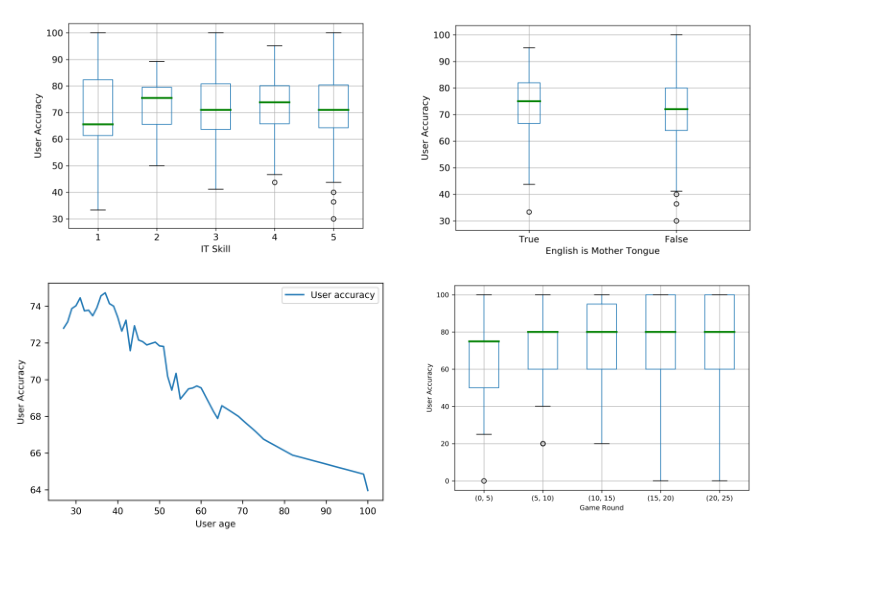
\includegraphics{Assets/ResultsHumanDetectionDeepFake.png}
 \caption{Menschliche Wahrnehmung von Audio Deepfakes (\cite{Mueller2022})}
 \label{fig:ResultsDetectionDeepfake}
\end{figure}
Die Teilnehmer wurden an Faktoren wie Alter, IT-Erfahrungen und Muttersprachler (die Studie wurde in englischer Sprache durchgeführt) kategorisiert.
Unter Abbildung \ref{fig:ResultsDetectionDeepfake} sind die Ergebnisse zu erkennen, in denen die Genauigkeit der Erkennung dem jeweiligen Personenkreis gegenüber gestellt ist.
Muttersprachler haben Vorteile bei der Erkennung von Fakes gegenüber Fremdsprachlern.
Weiterhin sei die IT-Kenntniss irrelevant, mit zunehmendem Alter verschlechterte sich die Genauigkeit. 
In den Ersten Runden nimmt die Genauigkeit bei der Erkennung zu, stagniert dann aber nach etwa 20 Runden.
Schaffung der Förderung von zukünftigen Gegenmaßnahmen werden benötigt, da sich die Qualität der Audio-Deepfakes erhöht, die menschlichen Fähigkeiten zur Erkennung allerdings stagnieren (\cite{Mueller2022}).
\par
Zur Untersuchung, welchen sozialen Einfluss Deepfakes auf den Menschen haben, verbindet Hancock (\cite{Hancock2021}) das Verhalten des Menschen auf generelle Falschinformationen mit der Täuschung von Deepfakes.
Menschen sind, so Hancock, nicht gut darin Falschinformationen als solche zu erkennen.
Es wird dazu geneigt, eher an das zu Glauben was gesehen wird.
Das gefährliche an Deepfakes ist die manipulierte Kombination von z.B. Stimme, Mimik und Gestik.
Während einer dieser Faktoren schon schwierig als Falschinformation zu entlarven ist, verstärkt diese Kombination durch Vertrautheit der Wahrnehmung die Glaubhaftigkeit des Fakes (Vgl. \cite{Hancock2021}).
Durch Sensibilisierung lassen sich die Effekte schmälern, so vergleich Hancock es mit der Existenz von Spammails, deren Gefahr durch allgemeine Bekanntheit verringert ist.






